\documentclass[UTF8,a4paper,8pt]{ctexart} 

 \usepackage{graphicx}%学习插入图
 \usepackage{verbatim}%学习注释多行
 \usepackage{booktabs}%表格
 \usepackage{geometry}%图片
 \usepackage{amsmath} 
 \usepackage{amssymb}
 \usepackage{enumitem}
  \CTEXsetup[format+={\flushleft}]{section}
 %设置文章宽度
\geometry{textwidth=18cm}
 %设置页面布局
\pagestyle{plain}
\author{郑华}
\title{我的生活历程}

 %正文排版开始
 \begin{document} 
 	\maketitle
 		 \section{November - 11月}
 		 \paragraph{Day 13}
 		 终于完成了 OpenCV 的蚂蚁路径的查找,在开始的迷茫到 中途 寻找方法的过程,都是一种充满未知的探险, 刚开始完全不懂的看网页教程文本资料,很成功的将环境安装成功,但是到后来发现提取路径并没有想象的那么简单,首先要对图像提取,然后计算重点,然而开始再没有看视频引导时,怎么也没有这样的思路, 所以在刚开始的时候,有个人引导是非常重要的。尤其是新东西。
 		 
 		 今天中午的时候 听到魏拖的眼睛过了,替他高兴,首先要肯定他的努力,也要为他的那种精神感到高兴。这个朋友不错。我要加紧步伐,不要落后...等我。
 		 
 		 晚上在上数据挖掘的时候,收到了明天要 进行 蓝欧C语音编程大赛,高兴并期待。
 		 
 		 终于开始了我的文档生涯, 昨天和宣旭峰 成立了我们的兴趣小组-大数据,希望我们可以坚持下去,从中学习也从中提高自身技能,加油
 		 
 		 但是还有好多事没做,不要愁,高兴点,一步一步来,你可以的!
 		 
 		  \paragraph{Day 14}
 		  早上进行了 蓝欧杯 C语音技能大赛, 感觉还不错,不知道能进决赛不,但是希望可以进,发现其中的函数指针考察的还是比较多的;
 		  
 		  比完赛后 魏拓 陪我吃了饭,路上我们讨论了也不知道什么话题,反正就是静静的也感觉很正常的那种。
 		  
 		  下午我有课,上课中,耿晗 坐到了我的旁边,虽然隔着一条路,但是还是那么心动,虽说放下但始终放不下。如果她可以放下那份冷淡,我真的愿意跟她走到最后。
 		  
 		  在上课中途,李嵩告诉我如果 我不去干点活的话,都不知道怎么去吃饭时,但是这我一直没意识到这一点,但是他却记得很到位,感觉,这样可以为你考虑的朋友,有时真的不多,我需要向你学习,请教我,我会努力的,这就是情商,这就是兄弟的感情维持 方法。
 		  
 		  
 		  晚上,我们去吃饭了,就因为交了 林菁,然后王科对 李嵩和我 一顿痛骂,我们其实是想给他一种惊喜,可是结果偏偏总是与人想象的不同,然后李嵩回去了,留我一人在饭局,我一直一维他是第一个离开那个场面然后到饭局的,看来我还是不够了解他们,我没做到兄弟应该做的,
 		  
 		  晚上回来,继续我的记录。
 		  
 		  \paragraph{Day 15}
 		  起来时  已经11点了又,而且是魏拓和李嵩上来叫我时才起床的,怎么这么没有时间观念了。早上就这么过去了,希望以后能早起看晨光妩媚...
 		  
 		  下午来就开始 要进行数据挖掘的课程了,说实在的这课完全不知道在讲什么,完全没起到选课的效果。我要学会,但是我的心却不在这..我想开发游戏,图形学是我的必经过路,所以,我愿意学习。
 		  对于大数据说实在的,只是想了解,但是什么事情都不是绝对的,走一步说不定下一步就是上上步...
 		  
 		  上完课,我的时间在不知不觉的从指尖溜走,怎么总在干些无所事事的事~  请 集中注意力  干一件 现在必须要干的事!!
 		  
 		  晚上,给爸妈打了个电话,说说聊聊家常,其实,家里就我一个儿子,时不时给爸妈打个电话,年纪大了,才发现,陪他们的时间真的不多了, 我还没让你们享受我给你们的幸福, 我会更努力的让自己变得 更好,只有这样, 我才觉得,这可以弥补对你们对我的关心与养育之恩。 
 		  
 		  终于,C++的游戏开发找到 步骤了,这就是前几天总结的那样,朝着那个方向前行,有时可能方向错了,但是总会到达那个目的地的。所以一切只要脚踏实地 的 干 就行了。  
 		  
 		  做个实干家,做个理想家, 做个珍惜朋友的人, 做个有意思的人, 做个为别人着想的人, 做一个有点情商的人....
 		  
 		  \paragraph{Day 16}
 		  早上起来又11点了,生活怎么过的这么没有时间感呢。你可以早起的!!!
 		  
 		  中午来办公室后,下了Hadoop的视频 和 数据挖掘的视频,看了2集数据挖掘,在群里找了C++游戏的大神,聊了会儿,知道了引擎是怎么回事,原来就是一个集成开发环境唉。  
 		  
 		  晚上,看来一个游戏开发的视频,感觉前端其实可以做的,就是UI素材的收集可能比较难点。
 		  
 		  偶然,说帮一下中午发代码的那个人吧,没想到,真是见证了 “赠人玫瑰,手留余香”这句话的现实版本了,给了我很多代码,可以学习了。
 		  
 		  不知怎么,总是感觉今天过的不充实,QQ上花的时间太多了是问题的关键。
 		  \paragraph{Day 17}
 		  今天起的  还勉强可以,9点左右吧,看了一小会书,接着就是在玩手机,到底手机有什么要玩的,为什么就是不能离开床铺,走出宿舍进行奋斗呢
 		  ,生活应该再努力一点,再紧凑一点
 		  
 		  中午一起吃饭时,李嵩又在说色盲这事,可能是自己无法正视这个事实,心里很不舒服,还好他也理解。
 		  
 		  午饭后,回到实验室,看着色觉图,真挺担心的。
 		  
 		  下午时间过的很快,不知道干什么了都,时间就不知不觉的跑走了,又是QQ
 		  
 		  晚上洗完澡,回来,竟然不知道竟然开始了新的一门课,而且在下午的时候知道竟然应数也要考试了。在没有规划的情况下,确实事一下就聚到一起了。
 		  
 		  目前还有如下内容需要完成,请留心,一步一步来,可以的,不要急,本周11周
 		   \begin{itemize}[fullwidth,itemindent=2em]
 		   	\item - 12 周应数考试
 		   	\item - 12 周MySQL搭建
 		   	\item - 12 周MeiLi's Ants
 		   	\item - 12 周毛中特1000字论文
 		   	\item - 13 周JavaEE学习项目检查
 		   	\item - 13 周自然辩证法考试
 		   \end{itemize}
 		   
 		   \paragraph{Day 18}
 		   今天早上起的出奇的早,其实也不早,8:00了,李飞说了一句话,觉得很有道理-“一次起不来,就在难起来了”,以后争取下床,体会早起的乐趣。早上听了他们的开题报告,感觉还是很有感觉的,不懂自己如何开始自己的毕设之路,纠结
 		   
 		   中午,吃完饭,睡了会,跟着他们去取了东西,接着听报告,终于有个图像相关的东西,也许这就是我想要的~ 但是结果却很触目惊心,让我对自己的研究开始操心了~
 		   
 		   晚上,又是上课
 		   
 		   感觉今天又什么都没干
 		   
 		  \paragraph{Day 19}
 		  你好,郑华:
 		  
 		  对于今天,你觉得离你的目标远了还是近了,对于你今天的所做所为,你是否感到心安理得。今天的读书是否只是耍耍存在,完全没理解,你需要的是勇敢去做德精神,你需要的是日积月累的进步。
 		  
 		  把时间当朋友 这本书中的道理你是否看明白了,时间不是管理出来来的,而是通过每天日积月累的不断干事积累出来的。只要朝着一个方向前进,每天学一点,那么你就会到达的
 		  
 		  影响你一生的100个哲理 这书中的 读者甲 就是现在你的目标,同样是一个现在看似没有用的东西,那完全可能是自己的目光不够,学吧,反正技多不压身。你说呢 
 		  
 		  还有很多,每天积累一点,总会离那个路口走近一些
 		  
 		  加油,你会成为一个IT的传奇。
 		  
 		  日程什么的都去一边,今天反正我是知道了 :美丽sister是个大神,而且带着我可能会做运动匹配算法,这可能也是我的方向。而且图像建模也会学习的唉。 棒棒的,而且这些与游戏又有很多的相关联,这是我喜欢的,我会努力的,我会做一个可以让美丽姐 需要的人。
 		  
 		  每一件东西,你学了,总会在以后什么时候会用上的,所以,不要再报忧说这个那个学了没用哈,加油
 		  
 		  从改变心态开始~ 一步一步来,相信自己!
 		  
 		  \paragraph{Day 20}
 		  你好,郑华:
 		  
 		  终于体会到了早起的好处,你是不是要坚持下去将这一习惯发挥到最后。
 		  在早上别人睡觉的时候,我将美丽姐的账面进行了报销,对自己的快递进行了整理,将肠胃进行了清理。
 		  
 		  下午,多么领人激动的时刻终于要到了,在小宝和托托的陪伴下,我进到了杨凌区地方医院,这是我失败2次体检的地方,如果不是魏拓,我可能就真的放弃再来体检了,谢谢。  首先宝宝进去打听问了下图谱上的数字,然后是托托挡着测试的人群帮着我挨个的问,真的好感动,他们给了我勇气,虽然这是人生中的那么小的一个基点,单他却让我学到了很多,坚持原来可以这样理解~朋友原来就是这个时候给你打气的~
 		  
 		  回来后,终于像抛开了什么包裹一样,一身轻,完成一件事的感觉真的很棒
 		  
 		  下午让篮球运动进入了我的日程,酣畅的流汗夹杂着我的喜悦
 		  
 		  晚上在陪老范练习了会儿英语时,然后完成了积累已久的马克思作业,完成作业的感觉真好,我不想再拖着东西直到最后日期了,这样真的很煎熬。如果可以请每天干一点,积累积累,养成习惯,集中所有完成那件事。
 		  
 		  加油,你会成为一个IT的传奇。
 		  
 		  \paragraph{Day 21}
 		  早上起来时,也已经11点了,找到魏拓一起吃了饭,后来来到教室上课,上完课出去吃了个饭,花了100,回来偶然看到有人发了可以打字赚外快,然后就信了,然后进去交了99,又是99,中途的各种错语令我 有着急,有担心,有以为是上当受骗,到进入最后的中间的过程后,发现其实返还是假的,而工作是真的,其实现在的我也不知道,只是帖子上是这样说的,希望可以赚回来,然后,就有外快了。
 		  
 		  结果今天什么也没干,好像,晚上这个就花了1个晚上
 		  
 		  赚钱是不是现在不该考虑的事呢?但是赚点外快是好的,希望自己加油,能创造出一番辉煌
 		  
 		  总体上说,今天还没有开始应用数理的复习,但是马上就要开始考试了,加油,你可以的
 		  
 		  郑华:你会成为一个IT的传奇。
 		  
 	  \paragraph{Day 22  周日\&周记}
 		  过着同样的生活,相似的步伐却没有一点转变,如何才能优秀成为一个一直在问的问题而没有实际操作的事情。
 		  
 		  同样的早晨,同样的晚饭,不同的是我的日子又平淡的过了一天,没有创新,没有进步,没有什么突破
 		  
 		  挥霍的生活,迷茫的自己,生活的压力,学习的目标 一起看起来好复杂,好难办,有没有一步一步积累的解决方案呢
 		  
 		  疲惫的自己失去了明确的目标,失去了前进的方向,我想要的生活不是这样,我想要一个明确的目的地,而不是走一步算一步,我不想随风飘散。
 		  
 		  我的人生目标是什么呢,我的生活目标是什么,我的家庭目标是什么,一切的一切都是那么的不明确,难道抽个时间考虑下自己的未来就那么奢侈吗,这些看似很小的事情却影响这你生活而奋斗的热情,希望尽快的完成这些然后努力奋斗之
 		  
 		  平静的心情,平静的漫无感觉的僵尸,春天的寒风还是冬日的烈阳,没有一点活力,没有一点感觉,这不是想要的,那么想要就付出行动吧
 		  
 		  \subparagraph{周记}
 		  总体上的工作是这样的:
 		  	\begin{enumerate}[fullwidth,itemindent=2em,label=(\arabic*)]
 		      \item  MFC: 学习了一章,知道了MFC程序的运行原理和大体架构
 		      \item 书目:看完一本影响一生的100个哲理
 		      \item 兼职:报了一个打字的兼职,希望可以练习指法的同时挣点外快吧
 		      \item 毛中特:作业总算写完了
 		      \item OpenCV: 前一个蚂蚁的路径识别总算做完了,而且了解到自己也是干这个方向的了
 		      \item 数据挖掘:感觉这门课没起到要学的作用
 		      \item 应用数理:看了4页
 		      \item 游戏编程:认识了解了些东西,比如要学什么,然后怎么实践,现在处于第一阶段,学习MFC,认识了一个过来人,他给了些代码,谢谢
              \item 驾照体检:终于过了,谢谢姐~
 		    \end{enumerate} 	
 		    
 	    \paragraph{Day 23  周一 \  \ 阴天}
 		    一觉睡到了天大亮,12:30了,唉,怎么就成了这样,我也想拥有早起的快乐,能不能定下一个这样的目标,循序渐进呢
 		    
 		    今天总体上说,虽然没有什么工作进展,但是在做事方面还是值得鼓励的,至少在做一件事的时候没有想其他事,很专心,比如晚上上课。
 		    
 		    下午时候老师的劳务费终于要来了,庆幸但是同时也压力山大,希望可以好好工作,不要亏待这份人情,美丽姐真的是会为人,希望能从她身上学的更多吧,真的是机会啊
 		    
 		    四人帮的谈话,感觉没了话题,有什么解决方法\dots	其实这也是我的问题,如何寻找话题成为了我现在要解决的问题,答案在哪?	    
 		    
 		    \subparagraph{日程记录}
 		    \begin{itemize}[fullwidth,itemindent=2em]
 		    	\item 12:30-1:20  洗衣服+吃饭  
 		        \item 1:20\ -\ 3:00  报驾校\&事件完成\&
 		        \item 3:20\ -\ 4:50  图书馆,借书
 		        \item 5:00\ -\ 6:00  对着电脑,也不知道干了什么,时间就没了
 		        \item 6:00\ -\ 7:00  吃饭,拉屎
 		        \item 7:30\ -\ 9:00  认真的上课,今天这个课程听课值得表扬
 		        \item 9:00\ -10:00 打印陈志涛的应数作业
 		        \item 10:00-12:00 整理答案学习Latex数学排版
 		    \end{itemize} 	
 		    
                 坚持,你定会成为IT的传奇!
 		  
 	  \paragraph{Day 24  周二 \  \ 阴天}
 		   每天都在感慨一件事,时间好快啊,好像在上课时感慨时间好慢一般,但是现在真的体会到,时间的利用率真的不够啊。这是一个需要提高的方面~
 		   
 		   有些时候,可以做的强势一些,不要把软弱当成了习惯,那么你的底线会不断的降下来,到降无可降时,一切都有些棘手了。
 		   
 		   今天的注意工作还是集中在应用数理的复习上,可是问题还是一个接一个的出现,直到晚上才发现,原来PPT耐下心来看,还是很有帮助的唉。
 		   
 		   下午老范请了吃了一顿自助餐唉,好久没吃了,谢谢哈~
 		   
 		   晚上逃课看了一部电影《小王子》--“如果希望跟某人发生羁绊,交要有为期流泪的准备”深深的刺进心中
 		   
 		   今天很感慨啊!又没早起啊,加油,这是你明天的目标,一天比一天好就行了。慢慢来
 		   
 		    坚持,你定会成为IT的传奇!
 		    
 	   \paragraph{Day 25  周三 \  \ 阳光明媚}
 		   有些事你无法预测,也无法估计,总在某些时候出现,我的软弱成为了我家族的致命伤,
 		   
 		   我感觉和魏拓好像出现了一点小矛盾,当然,这样消极的想法我不想再有。
 		   
 		   下午,\textbf{林菁团-- 林菁,杨亚玲,吴禅悦,魏拓 帮我尝试了第一次视频敲码,打了足足3个小时},好几千字,如图\ref{fig:Code},
 		   \begin{figure}[h]
 		   	\centering
 		   	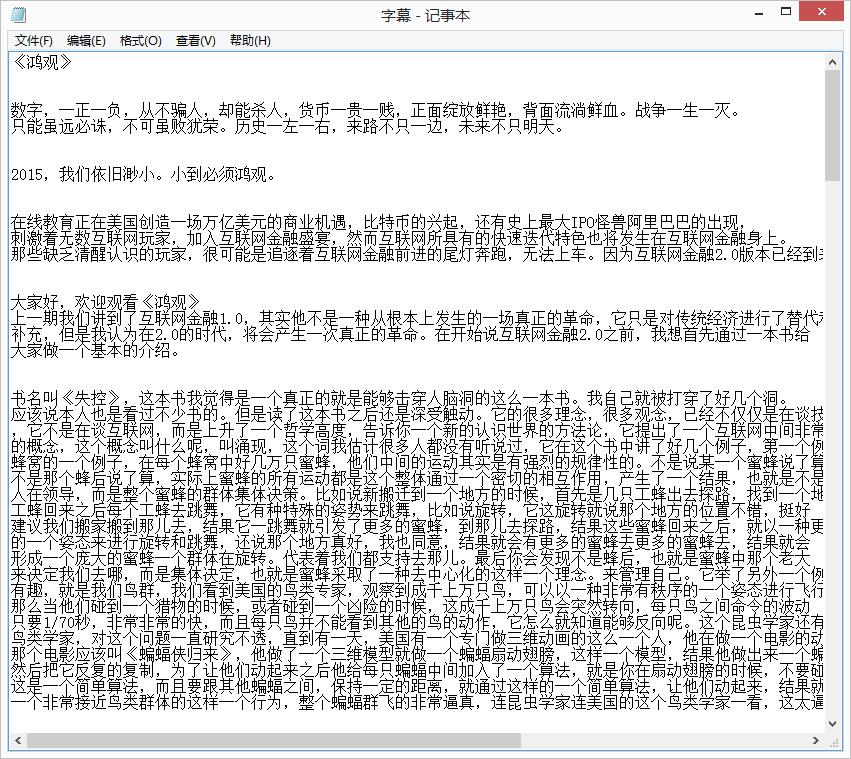
\includegraphics[width=8cm,clip]{20151125_Code.jpg} 	
 		   	\caption{打字留据}	
 		   	\label{fig:Code}
 		   \end{figure}
 		   
 		   却判定为正确率不足,很打击士气,但是希望这样的事不会出现第二次,我相信定会成功的逆袭。
 		   在此,向林菁,杨亚玲,吴婵玥,魏拓表示感谢。
 		   
 		   晚上,回去在存宝的指导下,学习了数学,深刻的体会到,\textbf{看到和想到的是无法替代真实的行动。}所以,请以行动为基准。
 		   
 		   还有,今天早上,老范起到了叫我早起的作用,完成了本周第一次早起$\big[9:30\big]$,谢谢
 		   
 		   早起的感觉真好,充满阳光的日子也非常令人兴奋与幸福。
 		   
 		     坚持,你定会成为IT的传奇!
 		     
 	 \paragraph{Day 26  周四 \  \ 阳光明媚}
 		 今天早起了算是吧$\big[8:30\big]$,主要跟着存宝到图书馆学习了一天的应用数学,感觉跟着一个人学就是不一样,要是一个人的话,早跑神n回了,
 		 
 		 还有最令人兴奋的是,美丽姐给了900元唉,幸福ing
 		 
 		 父母手头最近也紧,钱要不回来,所以我也不能老添乱,但是家里在这种情况下给了我3500,真的好感激他们,有你们真好,谢谢爸妈。
 		 
 		 晚上,洗完澡回来将凸优化的论文改吧改吧,还算有个样子。希望有个成绩吧。
 		 
 		 总之,今天专注而充实。加油,保持这个状态。
 		  
 		 坚持,你定会成为IT的传奇!
 		 
 		 
 	  \paragraph{Day 27  周五 \  \ 阳光明媚}
 	  
 	    你好,郑华:
 	    
 	    你为今天的生活满意吗,为什么呢?
 	    
 	    今天接着是存宝叫的床,起的还是相对的早的也8:50了,这两天的早上感觉上自习特别的专注,因为旁边做了一个存宝监督吗,难道自己连这点心都控制不住了。
 	    
 	    下午,接着上午的步尘,接着学习,然后在图书馆继续深造,可是这跟早上的效率有着天壤地别,也不知怎么,一个人总是被旁边的女生吸引,难道就不能好好学会习么。
 	    
 	    晚上第一次带实习,感觉好激动,好多问题,也学到了好多,感谢这次实现助教的机会,好好干,加油
 	    还有,又被老范请了一段饭,怎么可以老是这样,自己都不会了。不过记住这次了,下次一定还你~
 	    
 	    明天就要考试了,好期盼,好希望马上把这个事抛到脑后,然后正儿八经的学习我的开车,因为太想拿到驾照了$\sim$
 	    
 	    这些天感觉 自己都不知道自己真正的目标是什么了,还是盲目 的跟着考试走,但是过不了,连奖学金都没了,什么制度呀~
 	    
 	    别忘了,咱是要搞游戏开发的。别忘了咱们的路上还有好多东西要学$\sim$ 别松懈,加油
 	    
 	    坚持,你定会成为IT的传奇!
 	    
 	\paragraph{Day 28  周六 \  \ 雾霾漫天飞} 
 	    你好,郑华:
 	    
 	    终于到达了审判日,早上接着老步伐,在看数学题,然后呢,下午考试,感觉一塔糊涂。
 	    
 	    晚上回来陪美丽姐打了会儿羽毛球,然后心情有些放松,就这样~ 一天就完了。
 	    
 	    有点郁闷,唉,不过总算把这事抛在脑后了$\sim$
 	    
 	    \subparagraph{最近的事}还有最近的事都有下面这些,抓紧时间,积累就是一切$\sim$
 	    	\begin{enumerate}[fullwidth,itemindent=2em,label=(\arabic*)]
 	    		\item  MFC:实现蚂蚁爬行的界面程序。
 	    		\item  辩证法:即将考试,该准备了
 	    		\item  课程:现在只剩下组合数学和软件体系架构了
 	    		\item  软件著作权:是不是可以申请1、2个
 	    		\item  兼职:Java实习,打字
 	    		\item  驾照:车是不是可以练下了
 	    		\item  游戏准备:图形学、引擎、C++。
 		    \end{enumerate} 	
 		    
     \paragraph{Day 29  周日 \& 周记 \  \ 雾霾漫天飞} 
          你好,郑华:
          
          早上,老妈的电话打得很早,一种亲切$\sim$ 一种思念$\sim$
          
          这个实验室(303)的事还真多,说不定这就是收人钱财该有的售后服务,那么就好好接受这份工作。
          
          下午,到练车的地方学了会儿车,发现倒库的思路完全不是,跟想象中的完全不一样,感觉这样的学习你是完全学不会怎么倒车的和车感的$\sim$不过为了驾照我也是拼了。
          
          晚上,一个人的晚餐还是吃出来了些不一样的感觉$\sim$
          
          早上老妈说带的衣服和苹果,结果今天的车堵的感觉把老表弟给坑了$\sim$,对不起了,不过先谢谢你哈,下次能帮你就先帮你哈
          
          最近没有看书,感觉空荡荡的$\sim$来加点油去吧
          
          \subparagraph{周记}   
          这周的生活感觉就被一个概率论复习搞得不像样了,不过也让我学习到了一个好习惯,早起的习惯$\sim$如果可以坚持一个月那么这个好习惯就会陪我一生了是不是,加油坚持。
          
          不过从这次的复习也确实体会到了 \textbf{积累的力量是短时间无法比拟的 },这是一种需要不断践行的理论和人生体会$\sim$。
          
          周五当了人生第一次的助教,值得纪念下不是吗,发现原来自己学的东西是那么的不扎实,学的东西是那么浅显易懂,而且别从这些优秀的大二生的身上也深深的知道认真和不装逼是多么招人爱,牛逼的人不用说一样可以被发现,所以,\underline{能力这方面可以跟人学,但千万别逞强,切记一句话,人外有人,天外有天}。
          
          最近干的事简单易于记录:考试准备,并没有做什么为总目标而奋斗的事迹。
          
          不过总的一点,没有谁那一天就过的很充实,每天都是一天新的历程,让每天成为一个良好习惯积累的日子,学习充足,学习满足,学会创造乐趣
          
          加油,你定会成为IT的传奇!
          
      \paragraph{Day 30  Monday  \  \ 雾霾看不见手}
         你好,郑华:
         
         晚上陪美丽姐打了一晚上,接着陪老范吃了个饭,一天就过去了$\sim$
         
         日
         
         这最后一天过的$\sim$
 \section{December - 12月}	  
      \paragraph{Day 1  Tuesday  \  \ 阳光明媚}
      Hello,ZhengHua:
      
      今天都干了什么事情呢,做了什么开创性的事情没,做了什么挑战自己的事情没,做了什么自己不敢做的事情没。
      
      早上又睡醒的晚了,不过,对于晚起的你没有跟美丽姐吃饭吧$\sim$
      
      下午开始做美丽姐的界面程序了,就因为一个变量重名,改了一下午,这傻逼问题出的也是醉醉的。
      
      晚上老规矩,跟着美丽姐打羽毛球去了,全身的细胞到活动起来了,好爽
      
      现在是学习win-GDI的时候了,come on boy! Let's Go!!!
      
      坚持,你定会成为IT的传奇!
      
      \paragraph{Day 2  Wednesday \  \ }Hello,ZhengHua:
      
      今天都干了什么事情呢,做了什么开创性的事情没,做了什么挑战自己的事情没,做了什么自己不敢做的事情没。
      
      早上兴冲冲的在9点起来后,冲到实验室编码,各种原来碰到的问题,\textbf{没有存根又得重新寻找答案,在没有记录的生活这样的低效率已经成为限制自己前行的一种约束}。所以,这一切的一切,在失误中总结,在学习中了解前行,记录是一件终受益的事。
      
      晚上跟着魏拓一起吃饭(涮牛肚),味道很不错,也听到了很多真心对白,做人确实不能太贪眼前便宜,又的时候就得学会人前人后都得会做事,这样才可以不断的前行$\sim$
      
      晚上逃课被美丽姐逮了个正着,不过跟美丽姐混就是有肉吃,美丽姐给了一个拍子于我,谢谢哈
      
      吴禅悦会不会是那个人呢?不要急,先看看,不要再犯同样的错误了
      
       坚持,你定会成为游戏界的传奇!
      \paragraph{Day 3  Thursday  \  \ }
      Hello,ZhengHua:
      
       今天都干了什么事情呢,做了什么开创性的事情没,做了什么挑战自己的事情没,做了什么自己不敢做的事情没。
       
       早上的时候领导了新手机,感觉很爽,花钱的时候完全感觉不到挣钱的辛苦,唉
       
       风流的生活还在继续,可是学习的脚步已经落后了,抓紧时间抓回来吧
       
       梦开始的时候,我不希望夹杂着后悔
       
       泪,如果可以消失,有时不能换回更清楚的结果,但是坚实的过程决定着以后的路
       
       最近在坚持着每天打一小时羽毛球,日子很滋润,但是完全没有奋斗的身影。
      
      \paragraph{Day 4  Friday  \  \ }
       Hello,Zhenghua:
      
       今天都干了什么事情呢,做了什么开创性的事情没,做了什么挑战自己的事情没,做了什么自己不敢做的事情没。
       
       早上又没了。
       
       下午也算没了。只是到上岛吃了下牛排
       
       晚上带实习,确实学到了很多,谢谢这份工作,“\textbf{实习也在做笔记,提前做,态度}”
      
      \paragraph{Day 5  Saturday \  \ }
      你好,郑华:
      
      今天做什么了都,学到了什么,了解到什么新东西,为游戏学习积累了什么没,为以后做了什么准备没,你觉得今天过的值得吗
      
      看了一部电影《Fury Max》,还不错
      
      晚上看了一会 MFC,打了会儿羽毛球,就结束了今天,好没有成就感唉
      
      \paragraph{Day 6  Sunday  \  \ }
      
      你好,郑华:
      
      加油,不要再无所事事。
      
      早上,由于懒床被灌了一个不靠谱的罪名,不过确实值得反思,该如何才能体现出或做出靠谱的形象
      
      中午,在监考后,这些孩子总是充满了惊奇,没到半个小时就做完了唉
      
      晚上,出去吃了个北京古铜涮羊肉,还不错,又是魏拓请的,宝也请的吃了个汉堡,不过真的不错
      
      谢谢今天给我的人生,有时这种煎熬可能就是一种进步
      
      11.30分走出了第一步,开始了MFC项目的第一步,加油,You Can Do That!
      
      坚持,你定会成为游戏界的传奇!
      
       \paragraph{Day 7  Monday  \  \ }
       你好,郑华:
       
       开始了新的一天,却没有做出与众不同的开端,没有体会到早起的快乐,这不是我要做的。这周早起的记录挑战是4天,加油
       
       今天太无聊,竟然没有出现一点值得记得事情唉。
       
       \paragraph{Day 8  Tuesday \ \  阴天 }
       
       我都不想说你好了,不过,加油,我相信自己会度过这个 漫无成就的日子的
       
       
       \paragraph{Day 9  Wednesday \ \  阴天 }
       你好,华仔:
       
       洗完澡瞬间感觉好多了,原来,洗澡真的可以提神醒脑唉。
       
       晚上吃饭,走在路上,也感觉挺好
       
       今天看到了有人用 DirectX + C++ 做出的游戏框架,而且一般的大型游戏都是这个框架,很高兴,希望自己的努力以后可以找到归属。
       
       长风飞柳,烟花细雨
       
       我要变得不一样,我要变得更好
       
       
       诶,好像今天又是老范叫我起床的唉,谢谢哈$\sim$
       
       加油,你定会成为游戏界的传奇!
       
       \paragraph{Day 10 Thursday \ \ 阴天}
       Hello ZhengHua:
       
       今天过的还满意吗,
       
       早上起床13点左右,下午上了2小时自习,晚上回来一直神游状态,不过唯一的收获就是买到了一套很不错的游戏开发宝典,感觉很好,只不过需要自己加油
       
       加油,明天晚上有实习,后天下午要考试。
       
       \paragraph{Day 11 Friday \ \ 阴天}
       
       你好,早上依旧没了起床的目标和动力,渐渐的失去了生活的动力
       
       下午,在办公室看了会儿书,还算学了会儿吧
       
       中午的时候,取了浅墨-毛星云的书,看着别人22岁之前干的事,然后看着自己的,瞬间觉得弱爆了都
       
       不过他的笔记告诉了我很多,受益匪浅,谢谢,我一定会达到这个最终开发游戏的目标的
       
       除此之外,我发现,原来他的路原来就是我的模版,OpenCV + DirectX + 图像处理
       
       如果真的要从事游戏开发这方面的工作,那么我还需要从以下几个方面进行准备。
      
       \begin{enumerate}[fullwidth,itemindent=2em,label=(\arabic*)]
       	
       \item C++ STL 内部实现原理
       \item C++ Boost库
       \item C++ modue库
       \item C++ efficent 系列
       \item 网络编程
       
       \item 设计模式
       \item 软件架构
       
       \item 计算机图像学
       \item 3D 数学
       \item DirectX
       \item MFC 
       
       \item Photoshop
       \item Maya+3DMax
       
       \item Linux
       \item Lua 脚本
       \item Phython 脚本
       \item Shell 脚本
        	
       \end{enumerate}
       不过加油,你会成为游戏界的传奇的
       
        \paragraph{Day 12 Saturday \ \ 阴天+雪天}
        
        你好,华仔:
        
        终于考完试了,
        
        早上在宿舍学了会儿习,然后吃个饭中午午休一会儿,觉得精神瞬间就好了
        
        其实早起 + 午休可能是最高效的工作方式,坚持一个月试试
        
        晚上,跟着李嵩去吃了个饭,魏拓和存宝出去吃饭却没有喊一句,可能这就是拉帮结派的节奏,算了,心情就这样变得不好了
        
        明天开始我们的游戏计划吧,come on
        
        加油,你定会成为游戏界的传奇
        
         \paragraph{Day 13 SunDay \ \ 阴转晴 \ \ 14周截}
         
         你好,华仔:
         
         今天尝试了下早起 + 午睡的模式,感觉还不错,至少早起的感觉不错
         
         午饭的时候又是这样,没法说,要是从刚开始就习惯一个人何必再牵强的将就,我对常存宝和魏拓很失望
         
         中午跟李嵩到东北人家 吃了很不错的 孜然羊肉,很回味
         
         下午则听说了 辽宁2夫妇创办 张姐烤肉拌饭的故事:想法+生活+致富 很受触动,希望以后自己也能干件对家人也很温馨的事情让他们不用再为钱而计较
         
         晚上+早上 学习了MFC 的8集左右的东西吧,感觉很好,要的就是这样的成就感
         
         偶尔看了个电影:很多人都是在最后的关头失败的,希望自己能坚持到最后。
         
         \subparagraph{周记}
         
         总体说是一周比较压抑的时光,该找个东西释放释放了
         
        \paragraph{Day 15 Tuesday \ \  好可爱的太阳 }
        你好,华仔:
        
        昨天过的还是比较充实的,因为开始了自己规划好的lifePlan了,还可以
        
        今天就要批评下了,因为又是老问题,没起床
        
        下午调了一下午的代码还是没有跳出来这个问题“\textit{1>LIBCMT.lib(wwincrt0.obj) : error LNK2019: unresolved external symbol wWinMain referenced in function \_tmainCRTStartup
        1>D: \textbackslash Code\_Work\textbackslash C++\textbackslash DirectX\_01\textbackslash x64\textbackslash Debug\textbackslash DirectX\_01.exe : fatal error LNK1120: 1 unresolved externals}”,感觉好没收获
    
        晚上跟着美丽姐屁颠屁颠的去打羽毛球了,出现了一个技术很高的高手,这才意识到天外有天,人外有人的意思。
    
        晚上回来上课,感觉其实上课认真听挺好的
    
        上完课,陪存宝修眼镜,结果又没控制住手,一下又买了个100元的眼镜
    
	    找何鹏师兄解决以上问题时,他也不会,不过他教会我 用stackOverFlow,并且在创建项目时 直接就创建了一个可以直接用的写好的win 框架。唉,\textbf{问人有时真的收获到的不是时间上的减少,而且会学到别人解决问题的方法}
    
	    解决完这个问题,接着我的DirectX学习,
    
	    我会成为游戏界的传奇的 !
    
        \paragraph{Day 16 Wednesday \ \  好可爱的太阳 但我没早起}
        
        你好,华仔:
        
        今天就把那个代码调通后,进入了懒惰期又,
        
        下午没干,晚上玩了1晚上
        
        中午,魏拓请吃饭,下午,美丽姐和范玉玲请吃饭
        
        感觉没学到东西,今天
   
   \paragraph{Day 17 Thursday  \ \ 大晴天}
   
       你好,郑华:
       
       早上因为老范起来,感谢
       
       中午到驾校兴致勃勃的准备去学车,结果啥都没学成
       
       回来把论文翻译完了
       
       晚上打了3小时的球
       
       回来玩了1小时的游戏
       
       时间到了,要走了
       
       这日子过的都找不到我的目标在哪了
       
        \paragraph{Day 18 Friday  \ \ 大晴天}
        
        日:竟然能睡到2点,睡醒来就直接可以洗澡了,洗个澡还把手指弄破了,
        
        下午答辩,却不会谈吐,多么悲催啊
        
        晚上带实习,又是一个多彩多艺的年代啊,大一就开始接触Unity3D 了唉
        
        看来我得加把劲了,感觉一天天的过的完全没了方向
        
        
        要做到虽败犹荣,而不是不站而败
        
        加油
        
       \paragraph{Day 19 Saturday \ \ 阴天}
       
       就像是生活中的很多事情一样,学会它的最好办法就是一遍又一遍的实践,直到完全掌握。
       
       有一种落差是,你配不上自己的野心,也辜负了所受的苦难
       
       今天早上起的挺早,起床后学习了DirectX ,发现DirectX的渲染原来是可以的,只不过是win32 自动生成的代码不是视频中的代码,细心真的很有帮助
       
       中午叫了份外卖,吃了后,找了下C++ 的资料,发现了一个写的很好的博客
       
       下午吃完饭后,就不在学习了,玩了一晚上游戏
       
       不过,早起后,发现罪恶感就不在那么明显了
       
       \paragraph{Day 20 SunDay  \quad  管他妈的什么天气 }你好,生活就是这样,每天反思反思,你还配活在世上或配的上这身皮囊吗。
       
       今天睡起来,你猜几点了,他妈真是堕落成狗啊,16点离开宿舍,洗澡吃完饭后18点
       
       打个球,这个日子过的好快
       
       晚上回来再玩个游戏到22:00
       
       最后再学习两个小时的习,这日子
       
       \subparagraph{周记 15周截}
        
        渐渐的失去了动力,但还在艰难前行,这就是生活,昨天看到那句话“有一种落差是,你配不上自己的野心,也辜负了所受的苦难”
        
        为什么换个手机换成了这样,妈的
        
        不过周六的生活方式值得提倡,加油
        
        梦现在才开始,永远不迟,只要加把劲,\textbf{切记,哪怕现在多学一分钟也比不学强!}
        
        对了,前几天定了份时间表,我要坚持养成习惯,以此为见
        
       \begin{figure}[h]
       	\centering
       			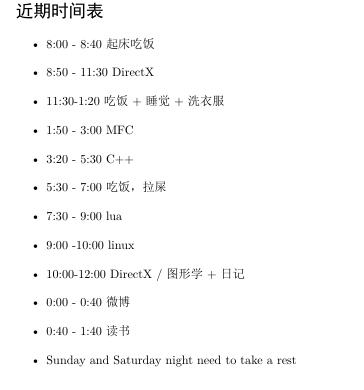
\includegraphics[angle=0,width=8cm]{Schedule.jpg}%就在前面括号中写图片名
       			\caption{时间表}
       			\label{fig:schedule}
       		\end{figure}%
       		
       \paragraph{Day 21 Monday  \quad  whatEver the weather is}
       
       Hello Mr.HUA
       
       在看到牛人的事迹后才觉得自己是那么的无能 还那么骄傲自负,“Linus花了两周时间自己用C写了一个分布式版本控制系统,这就是Git!一个月之内,Linux系统的源码已经由Git管理了!牛是怎么定义的呢?大家可以体会一下”
       
       早上起床起不起来,那是因为自己对梦想的强度还不够
       
       中午来办公室已经14点30 了,不过对于学习的专心程度点个赞
       
       晚上,现在的3人帮一起去吃了个黄记煌,
       
       回来玩游戏到22:00,开始学习到11:00
       
       最少知道了 游戏开发的框架是什么样了,引擎原来就是个C++项目然后转化成lib文件啊,那不就是一个类似于OpenCV 和DirectX 的库吗
       
       了解了GIT 的前生今世,很受感触,我还不是牛人,但会朝着那个方向去的。
       
       \paragraph{Day 22 TuesDay  \quad  反正也没出去,还管什么天气}
       
       早上10 点起的床,我发现,只要有一次就会有再三再四,唉,
       
       下次加油吧。
       
       每天重复着相同的把戏,反而没了动力
       
       打完球彻底没心情学习了。
       
       出去跟魏拓和存宝出去吃了个烧烤,心情还是可以的,就是回来后又在玩游戏,真的没自制力了啊
       
       打卡:
       \begin{enumerate}[fullwidth,itemindent=2em,label=(\arabic*)]
       	\item  8:30 前早起 \quad  No
       	\item  9:00 后的DirectX \quad No
       	\item  2:00 后的C++ \quad Yes
       	\item  6:00 后的Lua  \quad No
       	\item  8:00 后的图形学 \quad No
       	\item  0:50 后的读书 \quad Yes
       \end{enumerate}
       
      \paragraph{Day 23 Wednesday  \quad  霾,但心情挺好}
        Hello,Mr.HUA
        
        早上在起床与接着睡的挣扎中,终于成功的战胜了一次床。
        
        8:44 吃完饭并且来到了办公室,学了一早上DirectX11,并且很成功的体会到了早起的乐趣
        
        中午,尤文浩请吃了牛肉泡馍,老同学就是不一样,一顿饭就收买了
        
        下午回去看了会儿书,到13:25 吧,睡到15:00 洗澡,然后就到17:00了,定个场地,吃个饭,再陪老范出去买点水果,
        
        晚上打了一晚上游戏,但是早上控制住了,但晚上怎么就没控制住呢
        
        还有,下午一个人吃饭,碰到他们一起去的,感觉怪怪的,其实做最真实的自己挺好的。
        
            打卡: 
            \begin{enumerate}[fullwidth,itemindent=2em,label=(\arabic*)]
            	\item  8:30 前早起 \quad  Yes
            	\item  9:00 后的DirectX \quad Yes
            	\item  2:00 后的C++ \quad No
            	\item  6:00 后的Lua  \quad No
            	\item  8:00 后的图形学 \quad No
            	\item  0:50 后的读书 \quad Yes
            \end{enumerate}
       \paragraph{Day 24 Thursday  \quad 下午的太阳还可以}
        
        Hello,Mr.HUA
        
        早上也是起的异常的早,14:00 到达办公室吧,下午学习了一下午c++ ,把虚继承好好搞明白了下。
        
        晚上出去和 魏拓,常存宝,李飞,尤文浩,许红波一起去吃了小肥羊
        
        接着出去和 陈志涛,李嵩,晓东,杨宁,耿晗等一起唱了会儿歌
        
        总的来说,平安夜还是过的不错的。
        
       \paragraph{Day 25 Friday  \quad 太阳还可以}
       
       Hello, Mr.HUA
       
       感觉最近两天没有看DirectX诶,而且 马上考试了诶
       
       最近要交的作业有 数据库,数据挖掘等。
       
       要考的试有 马克思,组合数学,驾校科目一
       
       压力山大
       
       今天反而没起来,不知到自己能否坚持自己订的计划。我感觉哈佛的凌晨4点是非常值得一看的
        
        
         \paragraph{Day 26 Saturday  \quad 太阳还可以}
         
         今天真是放松了一天。
         
         玩了一天的游戏。
         
         \paragraph{Day 27 Sunday \quad 灰蒙蒙的太阳}
         
         Hello, MR.HUA
         
         今天9点被存宝叫起床,然后陪同魏拓看受伤的脚,接着跟着魏拓蹭了顿饭,就到下午16:00了,回来睡个觉,就到8:00了,洗了个澡就到22:00了,然后做了几百道题,就到1:00左右了。
         
         日子很简单,但是事情却很有意义。
         
           \subparagraph{周记 \quad 16周截}
           
           本周主要以玩为主,学习进度缓慢。
           
        \paragraph{Day 28 Monday \quad 太阳还可以}
        Hello,HUA
        
        今天把所有的科目一的题都做完了,明天就要考试了,希望能1次过吧。
        
        下午把数据挖掘的论文终于写完了
        
        晚上打了一晚上游戏。
        
        希望自己明天好运吧。
        
        去年的今天是刚考完研究生吧,今年这两天却在一直玩游戏$\sim$
        
       \paragraph{Day 29 Tuesday  \quad  灰蒙蒙的天}
       
        Hello,HUA:
        
        科目一过了哈。
        
        晚上照常堕落,不过明天回去后希望能获得点指教吧。
        
      \paragraph{Day 30 Wednesday  \quad 晴朗}
      
      Hello,郑华:
      
      今天带着希望回家看爸妈了,依旧是那样的想着我。可是就待了一个晚上就走了,老爸还是为贷款要不回而烦恼,老妈则在一边开导。
      
      日子好简单,也好惬意。
      
      \paragraph{Day 31 Thursday \quad 晴朗}
      
      早上老爸起来做了饭,中午妈就从学校回来专门为我做了顿饭,下午还没来得及说走就走了。
      
      陪着老舍友们一起吃了泡馍,就坐着安伟的车到小白家了,
      
      晚上先是KTV,然后是回来睡觉,觉睡的并不是很称心如意
      
      然而这一年就这样过去了。
      
      
\end{document} 
 		    